\documentclass[12pt,a4paper]{article}

\usepackage[UTF8]{ctex}
\usepackage{amsmath,amssymb,amsthm}
\usepackage{mathtools}
\usepackage{graphicx}
\usepackage{tikz}
\usepackage{hyperref}
\usepackage{geometry}
\usepackage{enumitem}
\usepackage{tcolorbox}
\tcbuselibrary{theorems}

\geometry{margin=2.5cm}

\theoremstyle{plain}
\newtheorem{theorem}{定理}[section]
\newtheorem{proposition}[theorem]{命题}
\newtheorem{corollary}[theorem]{推论}
\newtheorem{lemma}[theorem]{引理}

\theoremstyle{definition}
\newtheorem{definition}[theorem]{定义}
\newtheorem{example}[theorem]{例}
\newtheorem{problem}[theorem]{问题}

\theoremstyle{remark}
\newtheorem{remark}[theorem]{注记}
\newtheorem{conjecture}[theorem]{猜想}

\title{\bfseries Turán 定理与平面镶嵌图形\\——以正方形铺砌为例}
\author{}
\date{\today}

\begin{document}

\maketitle

\begin{abstract}
本文探讨将极值图论中的 Turán 定理应用于平面镶嵌（铺砌）问题的可能性。
以正方形铺砌为具体研究对象，定义铺砌的\textbf{接触图}，分析其图论性质（平面性、最大度、禁用子图），
并讨论``重边''概念的合理推广——带权接触与多重接触段。
最后提出若干可供进一步研究的问题。
\end{abstract}

\tableofcontents

% ============================================================
\section{Turán 定理回顾}
% ============================================================

\begin{definition}[Turán 图]
设 $n,r$ 为正整数，$r \le n$。\textbf{Turán 图} $T(n,r)$ 是 $n$ 个顶点的完全 $r$ 部图，
其各部的大小尽可能相等，即各部大小为 $\lfloor n/r \rfloor$ 或 $\lceil n/r \rceil$。
\end{definition}

记 $T(n,r)$ 的边数为 $t(n,r)$。则
\begin{equation}\label{eq:turan-edge}
t(n,r) = \left(1 - \frac{1}{r}\right)\frac{n^2}{2} + O(n) .
\end{equation}
精确公式为：设 $n = qr + s$，$0 \le s < r$，则
\[
t(n,r) = \binom{r}{2} q^2 + s(r-1)q + \binom{s}{2}.
\]

\begin{theorem}[Turán, 1941]\label{thm:turan}
设 $G$ 是 $n$ 个顶点的简单图。若 $G$ 不含 $K_{r+1}$ 作为子图，则
\[
|E(G)| \le t(n,r),
\]
等号成立当且仅当 $G \cong T(n,r)$。
\end{theorem}

直观上，Turán 定理是说：\textbf{要避免出现大小为 $r+1$ 的团，最``稠密''的做法是把顶点尽可能均匀地分成 $r$ 个部分，
各部分内部无边，部分之间全连边。}

\begin{remark}
本文最关心 $r=4$ 的情形：不含 $K_5$ 的图边数至多为 $t(n,4) \approx \frac{3}{8}n^2$。
\end{remark}

% ============================================================
\section{铺砌的接触图}
% ============================================================

\subsection{定义}

\begin{definition}[铺砌]
平面 $\mathbb{R}^2$ 的一个\textbf{铺砌}（tiling / tessellation）是一族紧致区域 $\{T_1, T_2, \dots\}$（称为\textbf{瓷砖}），
满足：
\begin{enumerate}[label=(\roman*)]
    \item 瓷砖的内部两两不交；
    \item 瓷砖的并集覆盖整个区域（或给定区域）。
\end{enumerate}
本文主要考虑\textbf{正方形铺砌}：所有瓷砖均为轴对齐或任意方向的正方形，尺寸可以不同。
\end{definition}

\begin{definition}[接触图]\label{def:contact}
铺砌 $\mathcal{T} = \{T_1, \dots, T_n\}$ 的\textbf{接触图}（contact graph）$G(\mathcal{T})$ 定义为：
\begin{itemize}
    \item 顶点集 $V = \{v_1, \dots, v_n\}$，$v_i$ 对应瓷砖 $T_i$；
    \item 边 $v_i v_j$ 存在当且仅当 $T_i$ 与 $T_j$ 的边界交集包含长度为正的线段，即
    \[
    \dim_{\mathcal{H}}\big(\partial T_i \cap \partial T_j\big) = 1 .
    \]
    （即两瓷砖共享一段非退化的边界段。）
\end{itemize}
\end{definition}

\subsection{平面性与最大度}

\begin{proposition}[接触图是平面图]\label{prop:planar}
任意平面铺砌的接触图都是平面图。
\end{proposition}
\begin{proof}
取每块瓷砖内部一点作为顶点，沿共享边界段的中点连线作为边，可得到接触图的一个平面嵌入。
由于瓷砖内部不交，这些边不会交叉。
\end{proof}

\begin{proposition}[最大度]\label{prop:degree}
对于由凸 $k$ 边形构成的铺砌，接触图的最大度 $\Delta \le k$。
特别地，正方形铺砌的接触图中 $\Delta \le 4$。
\end{proposition}
\begin{proof}
每块凸 $k$ 边形至多有 $k$ 条边，每条边至多与一个邻居共享（边对边铺砌）
或至多与有限个邻居共享（非边对边情形，但每条边上接触的邻居仍在接触图中贡献度数）。
凸性保证每个邻居占据每条边上至多一段。
\end{proof}

\subsection{禁用子图与 Turán 比较}

因为接触图是平面图，由 Kuratowski 定理知它不含 $K_5$ 及 $K_{3,3}$ 细分。
特别地，正方形铺砌的接触图\textbf{不含 $K_5$}。由定理~\ref{thm:turan}（$r=4$），
$n$ 块瓷砖的接触图边数 $m$ 满足
\begin{equation}\label{eq:turan-bound}
m \le t(n,4) \approx \frac{3}{8}n^2 .
\end{equation}

然而，平面图的边数有更紧的界 $m \le 3n-6$（$n \ge 3$），远小于 $O(n^2)$ 的 Turán 界。
因此 Turán 定理在此直接应用得到的界\textbf{远弱于平面性本身}。

但 Turán 定理的意义在于：它给出了\textbf{仅凭 $K_{r+1}$ 禁用} 就能推出的最优边数上界。
换言之，如果我们放弃``可平面嵌入''这一几何约束，仅保留``某些团被禁止''的组合条件，
Turán 定理给出了在此放松框架下的极值。

% ============================================================
\section{``重边''的合理推广}
% ============================================================

\subsection{为什么真正的重边不存在}

对于正方形（一般而言，任何凸多边形）铺砌，两枚瓷砖的交集 $\partial T_i \cap \partial T_j$ 是两个凸集的交，
因而也是凸集。在 $\mathbb{R}^2$ 中，两个凸多边形边界的交集只可能是：
\begin{itemize}
    \item 空集（不相邻）
    \item 一个点（仅角接触）
    \item 一条线段（沿边接触）
\end{itemize}

因此，\textbf{任意两枚正方形之间至多共享一条连续的边界线段}。
在简单图的框架下，这一对瓷砖之间至多贡献一条边，不存在传统的``重边''（multi-edge）。

\subsection{推广一：带权接触图}

如果不仅关心``是否接触''，还关心``接触多少''，则可定义\textbf{带权接触图}：
\begin{definition}[带权接触图]
在接触图 $G(\mathcal{T})$ 上赋予边权
\[
w(v_i v_j) = \big|\partial T_i \cap \partial T_j\big|_{\mathcal{H}^1}
= \text{两瓷砖共享边界的长度（1维 Hausdorff 测度）}.
\]
\end{definition}

此时 Turán 型问题变为：\textbf{要求不含某种带权子结构时，总权重 $\sum_e w(e)$ 的最大值是多少？}

\begin{example}
对于单位正方形铺砌（如棋盘格），每枚瓷砖有 $4$ 个邻居，每条边权重 $=1$（单位边长），
总和 $= 2n - 2\sqrt{n}$ 量级（考虑边界效应）。
而对于不等大小的正方形铺砌（如完美正方形剖分），权重分布则不均匀。
\end{example}

\subsection{推广二：非边对边铺砌中的多重接触段}

在\textbf{非边对边铺砌}（non-edge-to-edge tiling）中，可能出现这样的情况：
瓷砖 $T_i$ 的一条边与邻居 $T_j$ 的一部分接触，而同一条边的另一部分与邻居 $T_k$ 接触。
此时 $T_i$ 在同一边上有多个不同的邻居。

更精细地，若把每块正方形四条边各自视为独立的``半条边''（左右），则可以定义\textbf{接触段图}：
\begin{itemize}
    \item 顶点 = 每块瓷砖的每条边；
    \item 边 = 两条瓷砖边彼此接触（共享正长度）。
\end{itemize}
这是一个二部图（左右两侧各为同一边的接触关系），且每个顶点度数至多为 $1$（匹配约束）。

在此意义下，\textbf{同一对瓷砖可能在不同边上同时接触}——这便是``重边''或``多重边''的自然体现！
例如，一枚大正方形与一枚小正方形可能在两个不同的边上都有接触（小正方形被大正方形的拐角``嵌入''）。

\begin{center}
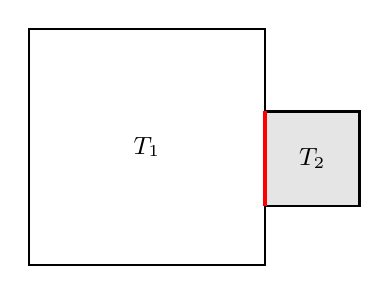
\begin{tikzpicture}[scale=1.5]
    % Large square
    \draw[thick] (0,0) rectangle (2,2);
    % Small square touching two sides
    \draw[thick,fill=gray!20] (2,0.5) rectangle (2.8,1.3);
    \node at (1,1) {\small $T_1$};
    \node at (2.4,0.9) {\small $T_2$};
    % Highlight contacts
    \draw[very thick,red] (2,0.5) -- (2,1.3);
    \draw[very thick,blue] (2,0.5) -- (2,0.5);  % just a mark
\end{tikzpicture}
\end{center}

更典型的例子：

\begin{center}
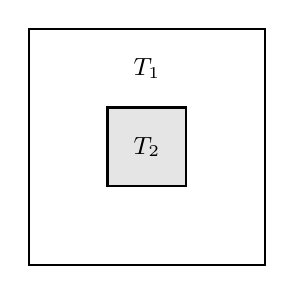
\begin{tikzpicture}[scale=1.0]
    % Large square
    \draw[thick] (0,0) rectangle (3,3);
    % Small square in a "corner pocket"
    \draw[thick,fill=gray!20] (1,1) rectangle (2,2);
    \node at (1.5,1.5) {\small $T_2$};
    \node at (1.5,2.5) {\small $T_1$};
    % Arrows showing multiple contact zones
\end{tikzpicture}
\end{center}

但注意上述情况下 $T_1$ 和 $T_2$ 的边界交集仍是一条折线段（拐角处相接触），并不是两个分离的线段。
要获得真正的``多重接触段''，需考虑非凸瓷砖或三维空间。

\subsection{推广三：超图视角}

把每块瓷砖的四条边视为四个``半超边''，定义\textbf{接触超图}：
\begin{itemize}
    \item 超边 = 一组瓷砖在同一个点相遇（如正方形的四个角点处有四块瓷砖相遇）。
\end{itemize}
这对于研究非边对边铺砌中的角接触结构特别有用。

% ============================================================
\section{Turán 型问题在铺砌中的可能应用}
% ============================================================

\subsection{从全局约束到局部约束}

Turán 定理的核心是：\textbf{全局禁止某个团，推出边数的全局上界，且极值图具有整齐的部结构。}
如果将这一思想迁移到铺砌问题：

\begin{problem}[Turán 型铺砌问题]
给定正整数 $r$。设 $\mathcal{T}$ 是一族 $n$ 枚正方形构成的铺砌，
且其接触图 $G(\mathcal{T})$ 不含 $K_{r+1}$。问：
\begin{enumerate}[label=(\alph*)]
    \item 接触图边数的最大值是多少？
    \item 达到最大值的铺砌具有怎样的结构？
    \item 若进一步要求 $G(\mathcal{T})$ 同构于 $T(n,r)$，是否存在对应的几何实现？
\end{enumerate}
\end{problem}

\begin{remark}
问题 (c) 是几何实现问题：\textbf{Turán 图 $T(n,r)$ 能否实现为某种正方形铺砌的接触图？}
对于 $r=2$，$T(n,2) \cong K_{\lfloor n/2\rfloor, \lceil n/2\rceil}$，
而二部平面图的最大边数为 $2n-4$，$T(n,2)$ 边数为 $\approx n^2/4$，
远超过平面图容量，故 $n$ 稍大即不可实现。
\end{remark}

\subsection{带权极值问题}

对带权接触图，考虑：
\[
W(\mathcal{T}) = \sum_{e \in E(G)} w(e) = \text{铺砌中所有瓷砖间接触的总长度}.
\]

\begin{problem}
对 $n$ 枚面积之和固定的正方形铺砌，$W(\mathcal{T})$ 的最大值及极值铺砌的结构是什么？
\end{problem}

这类似于等周问题（isoperimetric problem）的离散变体：固定总面积，最大化接触边界总长。

\begin{conjecture}
在总面积固定、只有单位正方形的情况下，最大化总接触长度的排列是尽可能接近正方形的网格排列。
\end{conjecture}

\subsection{完美正方形剖分与接触图}

\textbf{完美正方形剖分}（perfect squared square）是用彼此不全等的正方形铺满一个大正方形。
其接触图具有丰富的组合结构，且与电阻网络、平面图的对偶性有深刻的联系
（Brooks--Smith--Stone--Tutte, 1940）。

\begin{proposition}
完美正方形剖分的接触图是平面三角化图（或其子图）的对偶。
特别地，它不含 $K_5$，边数 $\le 3n-6$，且面度与正方形尺寸相关。
\end{proposition}

Turán 定理对此的直接约束较弱，但可以从另一角度切入：
若将正方形按大小分``部''，则同部内正方形是否倾向于不相邻？

% ============================================================
\section{总结与开放问题}
% ============================================================

\begin{enumerate}[label=\textbf{Q\arabic*}.]
    \item \textbf{几何 Turán 问题}：对给定类型的瓷砖（正方形、正多边形等），
    接触图能实现哪些禁用子图约束？Turán 极值图 $T(n,r)$ 在哪些 $r$ 值下可几何实现？
    
    \item \textbf{带权 Turán 问题}：若边带有权重（接触长度），
    在禁用某带权团结构的条件下，总权重的极值是多少？
    
    \item \textbf{多重接触与超图}：将非边对边铺砌中的多重接触建模为超图或多重图后，
    有何极值组合结果？
    
    \item \textbf{三维推广}：三维空间中立方体堆砌的接触图（面接触）有何性质？
    此时重边（多面共享多个面片）确有非平凡实例。
    
    \item \textbf{与完美正方形剖分的联系}：完美正方形剖分的接触图
    能否用 Turán 型推理给出新的组合不变量？
\end{enumerate}

\vspace{1cm}
\begin{tcolorbox}[title=初步结论]
Turán 定理对于铺砌问题的直接约束受限于平面图的更强制约（$m \le 3n-6$），
因此纯 Turán 界 $O(n^2)$ 在此并不紧。然而，Turán 定理所提供的\textbf{思想框架}——
通过禁用子结构来控制整体密度，再通过极值结构的部划分来理解组合架构——
对铺砌问题仍有启发性。特别是：
\begin{itemize}
    \item 将瓷砖按几何属性（大小、方向、颜色）分``部''；
    \item 考察部内与部间的接触模式；
    \item 通过带权或无权的 Turán 型极值推理，约束或预测铺砌的全局几何性质。
\end{itemize}
``重边''在正方形情形虽不真正存在，但通过\textbf{带权图}和\textbf{超图}的推广，
可以自然引入，并为三维或非凸铺砌问题铺路。
\end{tcolorbox}

\end{document}
